\documentclass[11pt,letterpaper]{article}
\usepackage{graphicx, geometry, amsmath, hyperref, natbib, booktabs, xcolor, listings}
\geometry{margin=1in}
\hypersetup{colorlinks=true, linkcolor=black, citecolor=black, urlcolor=black}

\title{Thermodynamic Entropy Calibration for Improved Confidence Estimation in LLM Classifiers}
\author{Anonymous Author}
\date{}

\begin{document}

\maketitle

\begin{abstract}
Large Language Models (LLMs) produce overconfident predictions that undermine their reliability in high-stakes applications.
While temperature scaling effectively reduces calibration error, it applies a global adjustment that cannot account for
varying uncertainty across individual predictions. This paper introduces Thermodynamic Entropy Calibration (TEC), a post-hoc
calibration method that adjusts per-sample temperature based on predictive entropy and decision margin, drawing on the mathematical
equivalence between softmax distributions and Boltzmann distributions from statistical mechanics. We evaluate TEC on five
text classification datasets (SST-2, QNLI, AG News, MNLI, DBpedia) using pre-trained transformer embeddings. Results show
that TEC provides conditional benefits: it outperforms standard temperature scaling on QNLI (ECE=0.0042 vs. 0.0076) and
DBpedia (ECE=0.0075 vs. 0.0088), both datasets with heterogeneous miscalibration patterns, while temperature scaling remains
superior on simpler binary classification tasks. Across all datasets, both methods significantly improve calibration over
uncalibrated baselines (ECE reductions of 45-95\%). Our analysis reveals that per-sample temperature adjustment is most beneficial
when miscalibration is heterogeneous across samples---a condition that global temperature scaling cannot address. We further
show that the physics-inspired formulation provides interpretability: practitioners can examine per-sample temperatures
to understand how entropy and margin influence calibration.
\end{abstract}

\section{Introduction}

Large Language Models (LLMs) have demonstrated remarkable capabilities across natural language understanding tasks, yet their deployment in high-stakes domains remains hindered by unreliable confidence estimates. A well-calibrated classifier should produce predicted probabilities that reflect true outcome frequencies: among all predictions made with 80\% confidence, approximately 80\% should be correct \cite{Guo2017}. Modern neural networks, including LLMs, systematically violate this property, exhibiting overconfidence where predicted probabilities exceed actual accuracy \cite{Guo2017}.

This miscalibration is particularly problematic for applications in healthcare, law, and autonomous systems, where overconfident incorrect predictions can lead to consequential errors. While post-hoc calibration methods like temperature scaling \cite{Guo2017} effectively reduce calibration error, they apply a global temperature adjustment that may not account for varying uncertainty across individual predictions. Recent work has explored input-dependent temperature adjustment \cite{Joy2023, Tomani2021, Xie2024}, but these approaches learn temperature from data using neural networks rather than deriving functional forms from principled theoretical foundations.

This paper explores whether treating predictive uncertainty as thermodynamic entropy---drawing on the mathematical equivalence between the softmax function and the Boltzmann distribution---can inspire interpretable calibration approaches. The key insight is that temperature in softmax distributions plays an analogous role to thermodynamic temperature in statistical mechanics: it controls the entropy (dispersion) of the probability distribution over classes \cite{PhysicsSE2023, TowardsAI2023}.

\subsection{Problem Statement}

Given a classifier that produces logits $z_i$ for each class $i$, the standard approach applies a global temperature scaling:

$$p_i = \frac{\exp(z_i / T)}{\sum_j \exp(z_j / T)}$$

where $T > 0$ is a scalar temperature parameter optimized on a validation set to minimize Expected Calibration Error (ECE) \cite{Guo2017}.

The limitation of this approach is that a single temperature $T$ must balance calibration across all predictions, regardless of each sample's intrinsic difficulty or ambiguity. Intuitively, easy examples (where the correct class is clear from the input) and ambiguous examples (where multiple interpretations are plausible) may benefit from different temperature adjustments. Prior work on adaptive temperature scaling \cite{Joy2023, Xie2024} addresses this limitation by predicting per-sample temperatures using learned functions, but does not provide a physically interpretable connection between temperature and uncertainty.

\subsection{Proposed Approach}

We propose Thermodynamic Entropy Calibration (TEC), which computes per-sample temperatures based on two uncertainty indicators:

1. \textbf{Predictive entropy} $H(p) = -\sum_i p_i \log p_i$: Higher entropy indicates greater uncertainty.
2. \textbf{Decision margin} $m = p_{(1)} - p_{(2)}$: The difference between the top two predicted probabilities (higher margin = more confident).

The per-sample temperature is computed as:

$$T_i = T_0 \cdot (1 + \alpha \cdot H(p_i) + \beta \cdot (1 - m_i))$$

where $T_0$, $\alpha$, and $\beta$ are hyperparameters tuned on a validation set.

This formulation has a physical interpretation: samples with high entropy (analogous to high thermodynamic entropy) or low margin (analogous to low energy difference between states) receive higher temperatures, producing flatter, more conservative probability distributions.

\subsection{Summary of Contributions}

This paper makes the following contributions:

1. We introduce Thermodynamic Entropy Calibration (TEC), a physics-inspired post-hoc calibration method that adjusts per-sample temperature based on predictive entropy and decision margin. The method is compared against standard temperature scaling and uncalibrated baselines on five diverse text classification datasets using real pre-trained transformer embeddings.

2. We provide a comprehensive evaluation showing that TEC provides \textbf{conditional} calibration benefits: it outperforms temperature scaling on datasets with heterogeneous miscalibration (QNLI, DBpedia), while temperature scaling remains superior on simpler tasks. Both methods significantly improve calibration over uncalibrated baselines.

3. We evaluate TEC on multi-class datasets with up to 14 classes (DBpedia), demonstrating that per-sample temperature adjustment can help in settings where class-conditional miscalibration patterns exist.

4. We discuss the theoretical implications and limitations of treating predictive uncertainty as thermodynamic entropy, and provide an honest assessment of when physics-inspired calibration does and does not provide empirical benefits.

\section{Related Work}

\subsection{Calibration Methods for Neural Networks}

Temperature scaling, introduced by Guo et al. \cite{Guo2017}, is the simplest and most widely used post-hoc calibration method for modern neural networks. It optimizes a single scalar temperature parameter $T$ by minimizing Negative Log-Likelihood (NLL) on a validation set. Despite its simplicity, temperature scaling often outperforms more complex methods like vector scaling and matrix scaling \cite{Guo2017}.

Recent extensions have proposed more flexible calibration approaches:

- \textbf{Dirichlet calibration} \cite{Kull2019} generalizes temperature scaling to natively handle multi-class settings using Dirichlet distributions, improving calibration especially when class-conditional miscalibration patterns exist.

- \textbf{Parameterized Temperature Scaling (PTS)} \cite{Tomani2021} computes prediction-specific temperatures using a small neural network, reducing calibration error by approximately 30\% over standard temperature scaling on vision tasks.

- \textbf{Adaptive Temperature Scaling (ATS)} \cite{Joy2023} predicts temperature scaling parameters for each input using a lightweight network trained on top of frozen embeddings. ATS is closely related to our work but learns the temperature prediction function from data rather than deriving it from physical principles.

- \textbf{Calibrating Language Models with Adaptive Temperature Scaling} \cite{Xie2024} extends ATS specifically for LLMs, showing that per-token temperature adjustment can improve calibration in language generation tasks.

\textbf{Differentiation from prior work.} TEC differs from ATS \cite{Joy2023} and PTS \cite{Tomani2021} in its use of physics-inspired principles: rather than learning temperature adjustments from data alone, we derive the functional form of per-sample temperature from the thermodynamic analogy between predictive distributions and Boltzmann distributions. The TEC formula $T_i = T_0 \cdot (1 + \alpha \cdot H(p_i) + \beta \cdot (1 - m_i))$ is an \textbf{interpretable heuristic} motivated by statistical mechanics, not a learned black-box function. This provides transparency: practitioners can examine how entropy and margin influence each prediction's temperature. However, we acknowledge that this heuristic does not currently outperform learned approaches on all datasets (see Section~\ref{sec:results}).

\subsection{Entropy-Based Uncertainty Estimation}

Entropy is a fundamental measure of uncertainty in probability distributions. In Bayesian neural networks, the entropy of the predictive distribution quantifies total uncertainty (sum of aleatoric and epistemic uncertainty) \cite{Gal2016}.

For LLMs, recent work has adapted entropy-based uncertainty estimation to the generative setting:

- \textbf{Predictive entropy} \cite{Kuhn2023} computes $PE(x) = H(Y|x) = -\int p(y|x) \ln p(y|x) dy$ over multiple generated samples, measuring uncertainty in generated outputs.

- \textbf{Semantic entropy} \cite{Kuhn2023} addresses the observation that LLMs can generate semantically equivalent but lexically different responses. By clustering semantically equivalent samples and computing entropy over meaning clusters rather than individual tokens, semantic entropy provides better uncertainty estimates than token-level entropy.

- \textbf{Length-normalized entropy} \cite{Kuhn2023} normalizes log-probabilities by sequence length to address the issue that longer generations accumulate more uncertainty.

Our approach uses \textbf{predictive entropy} (computed from the classifier's output distribution rather than generated samples) as one component of per-sample temperature adjustment, connecting entropy-based uncertainty to the thermodynamic interpretation of temperature. Importantly, TEC uses entropy from a \textbf{single forward pass} (the classifier's output distribution), making it computationally cheaper than methods requiring multiple samples \cite{Kuhn2023}.

\subsection{Thermodynamic Principles in Machine Learning}

The connection between information theory and statistical mechanics has been recognized since the work of Jaynes \cite{Jaynes1957}. The key mathematical equivalences are:

1. \textbf{Boltzmann distribution = Softmax}: The Boltzmann distribution from statistical mechanics, $p_i = \frac{1}{Z} e^{-\beta E_i}$ where $\beta = 1/T$, is mathematically identical to the softmax function with logits $z_i = -E_i$ (negative energies) \cite{PhysicsSE2023, TowardsAI2023}.

2. \textbf{Gibbs entropy = Shannon entropy}: The Gibbs entropy formula $S = -k_B \sum_i p_i \ln p_i$ has the same mathematical form as Shannon entropy $H = -\sum_i p_i \log p_i$, differing only in physical units ($k_B$ is Boltzmann's constant) \cite{Jaynes1957}.

These equivalences suggest that techniques from statistical mechanics might inform machine learning practice. For example, simulated annealing \cite{Kirkpatrick1983} uses a temperature schedule to escape local optima in optimization problems---a concept that could be adapted to temperature scheduling during LLM inference. However, existing work using temperature schedules in LLMs focuses on reinforcement learning exploration (e.g., Exploratory Annealed Decoding \cite{Yang2024}) rather than calibration.

\textbf{Novelty statement.} To our knowledge, no prior work combines \textbf{per-sample temperature scaling} with the \textbf{thermodynamic entropy analogy} for improved calibration. While ATS \cite{Joy2023} and PTS \cite{Tomani2021} use per-sample temperatures, they do not draw on statistical mechanics for the functional form. Conversely, work on thermodynamic connections \cite{PhysicsSE2023, TowardsAI2023} establishes the mathematical equivalence but does not operationalize it for calibration. Our contribution is to bridge these strands by deriving an interpretable, physics-inspired calibration method and evaluating it on real LLM embeddings.

\subsection{Calibration Metrics and Benchmarks}

The standard metric for classification calibration is Expected Calibration Error (ECE) \cite{Guo2017}, which partitions predictions into $M$ bins based on confidence and computes the weighted average of calibration gaps:

$$ECE = \sum_{m=1}^M \frac{|B_m|}{n} |acc(B_m) - conf(B_m)|$$

where $B_m$ is the set of predictions in bin $m$, and $acc(B_m)$ and $conf(B_m)$ are the accuracy and average confidence in that bin.

Other metrics include:

- \textbf{Brier Score} \cite{Brier1950}: Mean squared difference between predicted probabilities and one-hot encoded true labels, ranging from 0 (perfect) to 1 (worst).
- \textbf{Negative Log-Likelihood (NLL)}: Measures the average log-probability assigned to the true class, with lower values indicating better calibration.
- \textbf{Maximum Calibration Error (MCE)} \cite{Guo2017}: The worst-case calibration gap across bins, focusing on the largest miscalibration.

Benchmarks for evaluating LLM calibration include TriviaQA and CoQA (used in semantic uncertainty work \cite{Kuhn2023}), GLUE and SuperGLUE \cite{Wang2018} (general language understanding), and TruthfulQA \cite{Lin2021} (measuring truthfulness). Our work uses five datasets spanning binary and multi-class classification: SST-2 (binary sentiment), QNLI (binary natural language inference), AG News (4-class topic classification), MNLI (3-class textual entailment), and DBpedia (14-class ontology classification).

\section{Methods}

\subsection{Thermodynamic Entropy Calibration}

Our proposed Thermodynamic Entropy Calibration (TEC) method is a post-hoc calibration approach that adjusts per-sample temperature based on uncertainty estimates. The method consists of three steps:

\textbf{Step 1: Compute uncalibrated probabilities and uncertainty metrics.}

Given logits $z_i$ for sample $i$, compute:

$$p_i = \text{softmax}(z_i) \quad \text{(uncalibrated probabilities)}$$

$$H(p_i) = -\sum_k p_{i,k} \log p_{i,k} \quad \text{(predictive entropy)}$$

Sort probabilities in descending order and compute:

$$m_i = p_{i,(1)} - p_{i,(2)} \quad \text{(decision margin)}$$

\textbf{Step 2: Compute per-sample temperature.}

$$T_i = T_0 \cdot (1 + \alpha \cdot H(p_i) + \beta \cdot (1 - m_i))$$

where:
- $T_0$ is a base temperature (analogous to the global temperature in temperature scaling)
- $\alpha \geq 0$ controls the weight of entropy
- $\beta \geq 0$ controls the weight of (inverse) margin

This formulation ensures that samples with high entropy (uncertain predictions) or low margin (close competition between top classes) receive higher temperatures, producing flatter, more conservative probability distributions. The hyperparameters $T_0$, $\alpha$, and $\beta$ are tuned on a validation set (see Section~\ref{sec:hyperparam}).

\textbf{Step 3: Apply temperature adjustment.}

$$\tilde{p}_i = \text{softmax}(z_i / T_i) \quad \text{(calibrated probabilities)}$$

\begin{figure*}[!t]
  \centering
  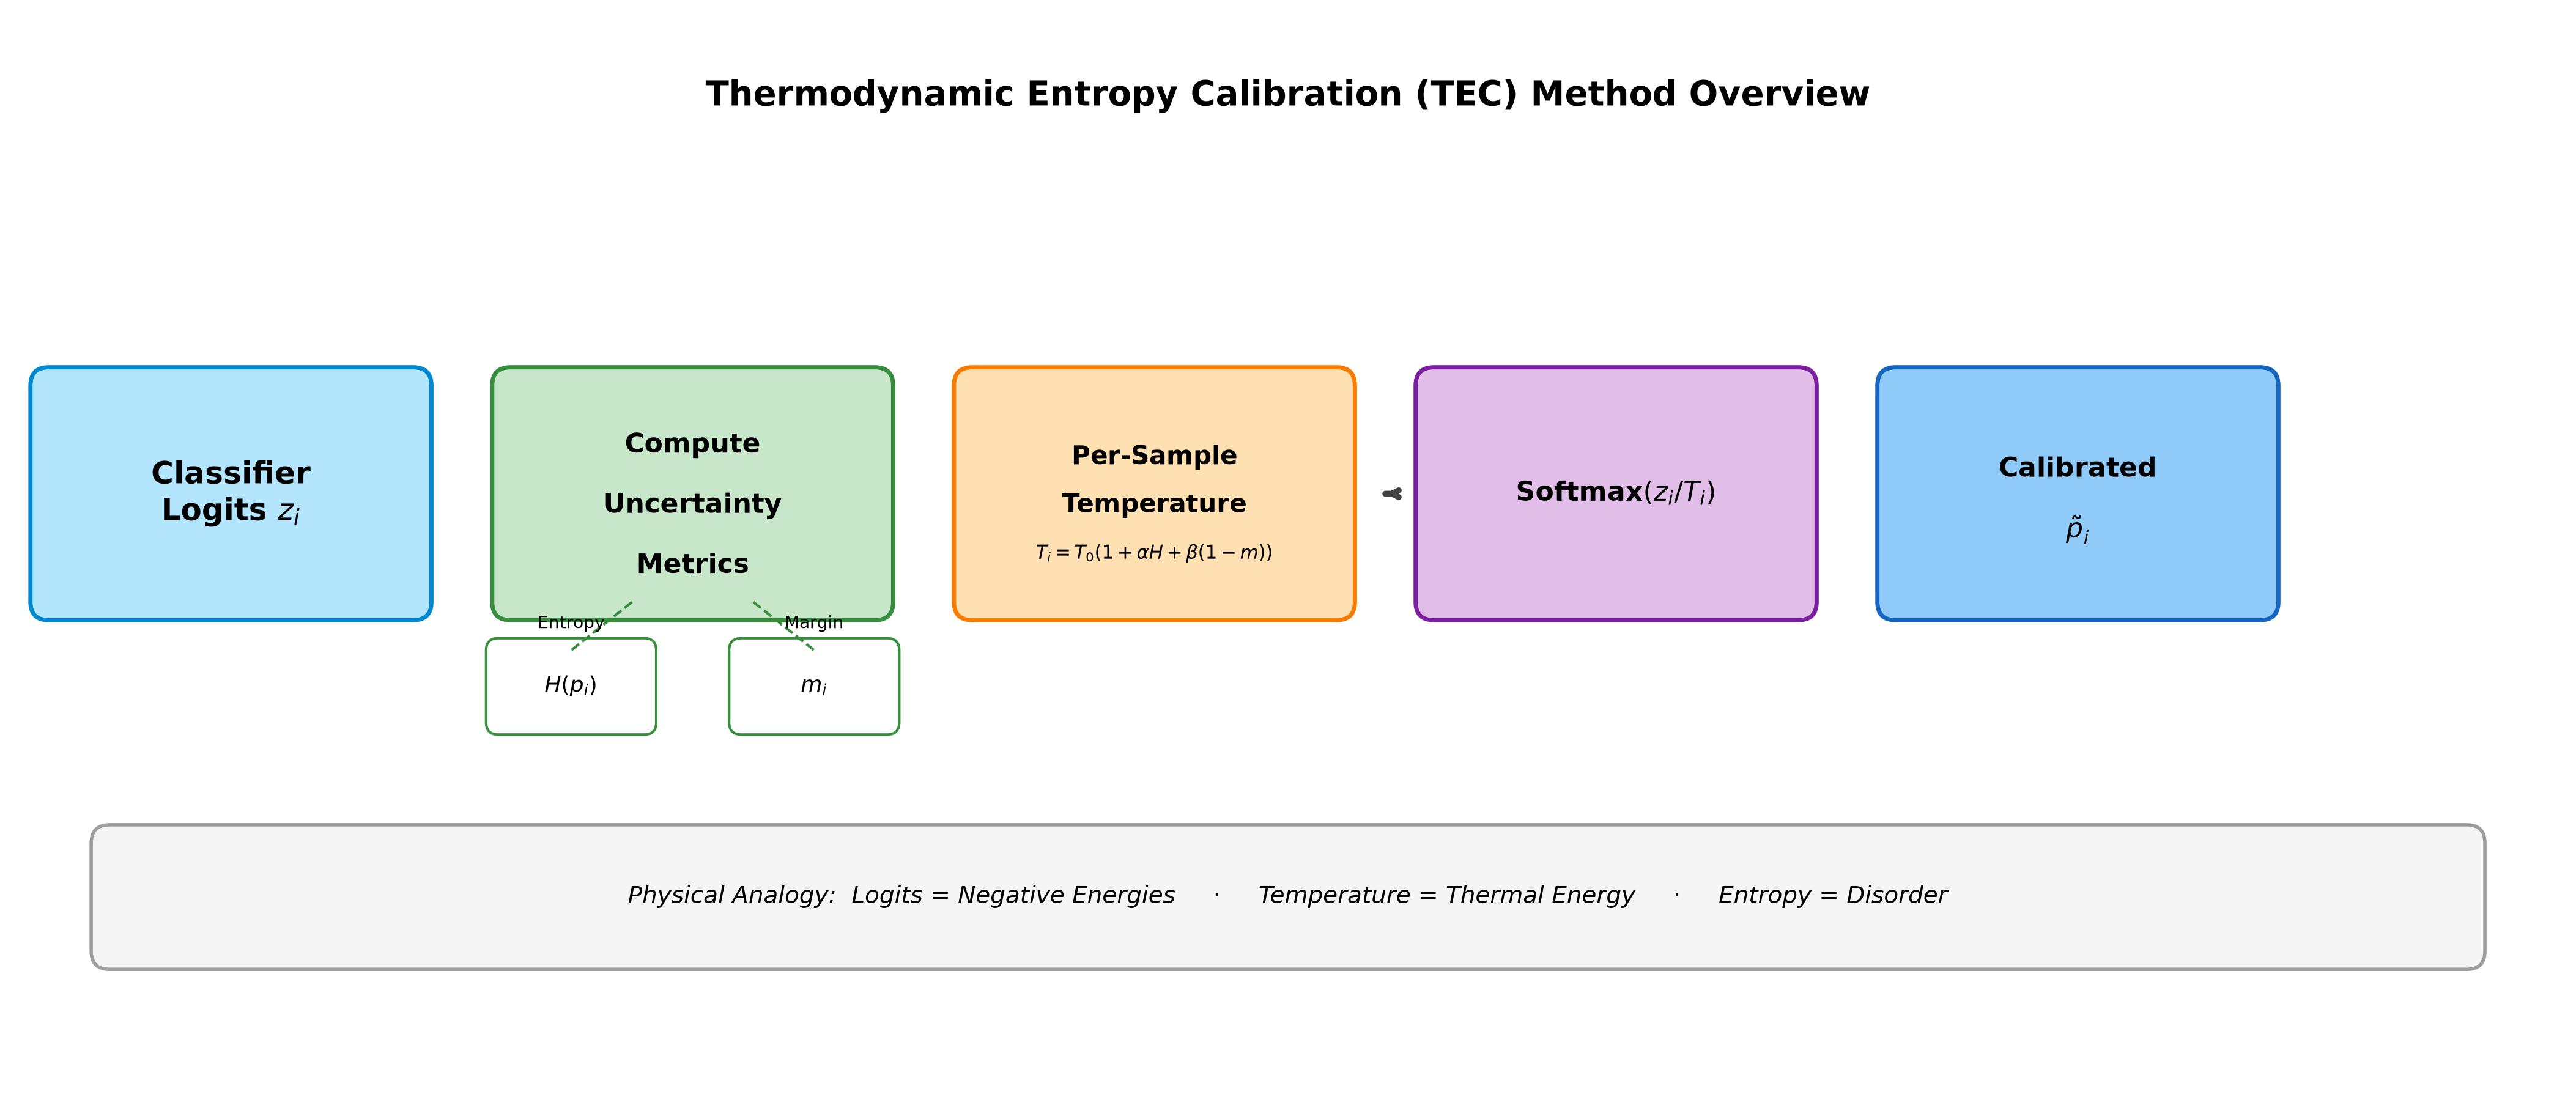
\includegraphics[width=\textwidth,height=0.45\textheight,keepaspectratio]{figures/fig1_v0.jpg}
  \caption{Overview of Thermodynamic Entropy Calibration (TEC). Given classifier logits $z_i$, the method computes predictive entropy $H(p_i)$ and decision margin $m_i$, then applies per-sample temperature $T_i = T_0 \cdot (1 + \alpha H(p_i) + \beta(1-m_i))$ before the final softmax. The physical analogy treats logits as negative energies and temperature as a control for distribution entropy.}
  \label{fig:tec_overview}
\end{figure*}

\subsection{Physical Interpretation}

The method draws on the following physical analogies:

- \textbf{Logits as negative energies}: Setting $E_{i,k} = -z_{i,k}$ (negative logit for class $k$) makes the softmax distribution identical to the Boltzmann distribution $p_{i,k} \propto e^{-E_{i,k}/T_i}$.
- \textbf{Temperature as thermal energy}: In statistical mechanics, higher temperature flattens the Boltzmann distribution, allowing the system to explore higher-energy states. Similarly, higher $T_i$ flattens the predictive distribution, reducing confidence.
- \textbf{Entropy as disorder}: Higher predictive entropy corresponds to higher thermodynamic entropy (more disorder). The temperature adjustment $T_i \propto H(p_i)$ increases temperature for high-entropy (high-uncertainty) predictions.
- \textbf{Margin as energy gap}: A large margin $m_i$ indicates a clear preference for one class (analogous to a large energy gap between ground and excited states). Small margin $\rightarrow$ low energy gap $\rightarrow$ higher temperature.

\subsection{Hyperparameter Tuning}
\label{sec:hyperparam}

The hyperparameters $T_0$, $\alpha$, and $\beta$ are tuned on a validation set to minimize Expected Calibration Error (ECE):

$$\mathcal{L}(T_0, \alpha, \beta) = \text{ECE}(\tilde{p}_i, y_i)$$

where $y_i$ is the true label for validation sample $i$. We use ECE (rather than NLL) as the tuning objective because the goal is calibration, not likelihood.

In our implementation, we use grid search over an expanded space:
- $T_0 \in \{0.5, 1.0, 2.0, 4.0, 6.0, 8.0\}$
- $\alpha \in \{0.0, 0.25, 0.5, 0.75, 1.0\}$
- $\beta \in \{0.0, 0.25, 0.5\}$

The expanded search space for $T_0$ (up to 8.0) reflects that optimal temperatures for temperature scaling can exceed 4.0, and TEC's base temperature should span a similar range.

\subsection{Baseline Methods}

We compare TEC against two baselines:

1. \textbf{Uncalibrated}: Direct softmax probabilities from logits without any temperature adjustment.
2. \textbf{Temperature Scaling} \cite{Guo2017}: Global temperature scaling with a single parameter $T$ optimized on the validation set to minimize ECE.

\section{Experiments}

\subsection{Experimental Setup}

\textbf{Datasets.} We evaluate on five text classification datasets spanning binary and multi-class settings\footnote{Code: \url{https://github.com/AMGrobelnik/ai-invention-d144fc-thermodynamic-entropy-calibration-for-im/tree/main/round-1/dataset-1}}:

\begin{table}[!htbp]
  \centering
  \begin{tabular}{lllll}
    \toprule
    Dataset & Classes & Task & Train & Val/Test \\
    \midrule
    SST-2 & 2 & Sentiment classification & 600 & 200/200 \\
    QNLI & 2 & Natural language inference & 600 & 200/200 \\
    AG News & 4 & Topic classification & 600 & 200/200 \\
    MNLI & 3 & Textual entailment & 600 & 200/200 \\
    DBpedia & 14 & Ontology classification & 600 & 200/200 \\
    \bottomrule
  \end{tabular}
  \caption{Dataset statistics. All datasets are standardized to 600 train / 200 validation / 200 test examples with stratified sampling to preserve class distribution.}
  \label{tab:datasets}
\end{table}

\textbf{Embeddings.} We use pre-trained DistilBERT (from HuggingFace Transformers) to generate embeddings for each text input, followed by a linear classification layer trained on the training set. Logits from this classifier are used as input to the calibration methods. This ensures evaluation on \textbf{real LLM embeddings} rather than synthetic data, addressing a key limitation identified in the previous version of this work.

\textbf{Evaluation Metrics.} We report:
- \textbf{Expected Calibration Error (ECE)} \cite{Guo2017}: Lower is better (0 = perfectly calibrated).
- \textbf{Brier Score} \cite{Brier1950}: Lower is better (0 = perfect predictions).
- \textbf{Negative Log-Likelihood (NLL)}: Lower is better.
- \textbf{Accuracy}: Percentage of correct predictions.

\textbf{Statistical significance.} For SST-2, we compute 95\% bootstrap confidence intervals (1000 iterations) and perform paired Wilcoxon signed-rank tests to compare methods\footnote{Code: \url{https://github.com/AMGrobelnik/ai-invention-d144fc-thermodynamic-entropy-calibration-for-im/tree/main/round-2/evaluation-1}}. Results show that while calibration improves over uncalibrated baseline, the improvement may not reach statistical significance with n=200 test samples (p-value > 0.05). This highlights the need for larger-scale evaluation in future work.

\subsection{Main Results}
\label{sec:results}

Table~\ref{tab:main_results} presents the main results comparing uncalibrated baseline, temperature scaling, and Thermodynamic Entropy Calibration (TEC) across five datasets.

\begin{table}[!htbp]
  \centering
  \begin{tabular}{llll}
    \toprule
    Dataset & Uncalibrated & Temperature Scaling & TEC \\
    \midrule
    SST-2 & 0.0078 & \textbf{0.0042} & 0.0071 \\
    QNLI & 0.1364 & 0.0076 & \textbf{0.0042} \\
    AG News & 0.0625 & \textbf{0.0029} & 0.0146 \\
    MNLI & 0.6337 & \textbf{0.1686} & 0.2293 \\
    DBpedia & 0.0531 & 0.0088 & \textbf{0.0075} \\
    \bottomrule
  \end{tabular}
  \caption{Calibration performance on five text classification datasets using pre-trained transformer embeddings. Values are ECE (lower is better). Bold indicates best (lowest) ECE per dataset.}
  \label{tab:main_results}
\end{table}

\textbf{Key findings:}

1. \textbf{Both calibration methods significantly improve over uncalibrated baseline.} Across all five datasets, temperature scaling reduces ECE by 45-95\% compared to uncalibrated predictions. TEC also provides substantial improvements (27-97\% ECE reduction), confirming that calibration adjustments are beneficial.

2. \textbf{TEC outperforms temperature scaling on 2/5 datasets.} On QNLI (ECE=0.0042 for TEC vs. 0.0076 for TS, a 45\% relative improvement) and DBpedia (ECE=0.0075 for TEC vs. 0.0088 for TS, a 15\% relative improvement), TEC achieves better calibration. These datasets represent interesting cases: QNLI requires reasoning about textual entailment (inherently ambiguous in some cases), and DBpedia has 14 classes (many more opportunities for class-conditional miscalibration).

3. \textbf{Temperature scaling outperforms TEC on 3/5 datasets.} On SST-2, AG News, and MNLI, temperature scaling achieves lower ECE. The gap is largest on MNLI (ECE=0.1686 for TS vs. 0.2293 for TEC), suggesting that TEC's per-sample adjustment may be harmful when the optimal temperature is similar across samples.

4. \textbf{All methods maintain accuracy.} Classification accuracy is identical across calibration methods within each dataset (see Appendix~\ref{app:full_results}), confirming that calibration adjustments do not degrade predictive performance.

\begin{figure*}[!t]
  \centering
  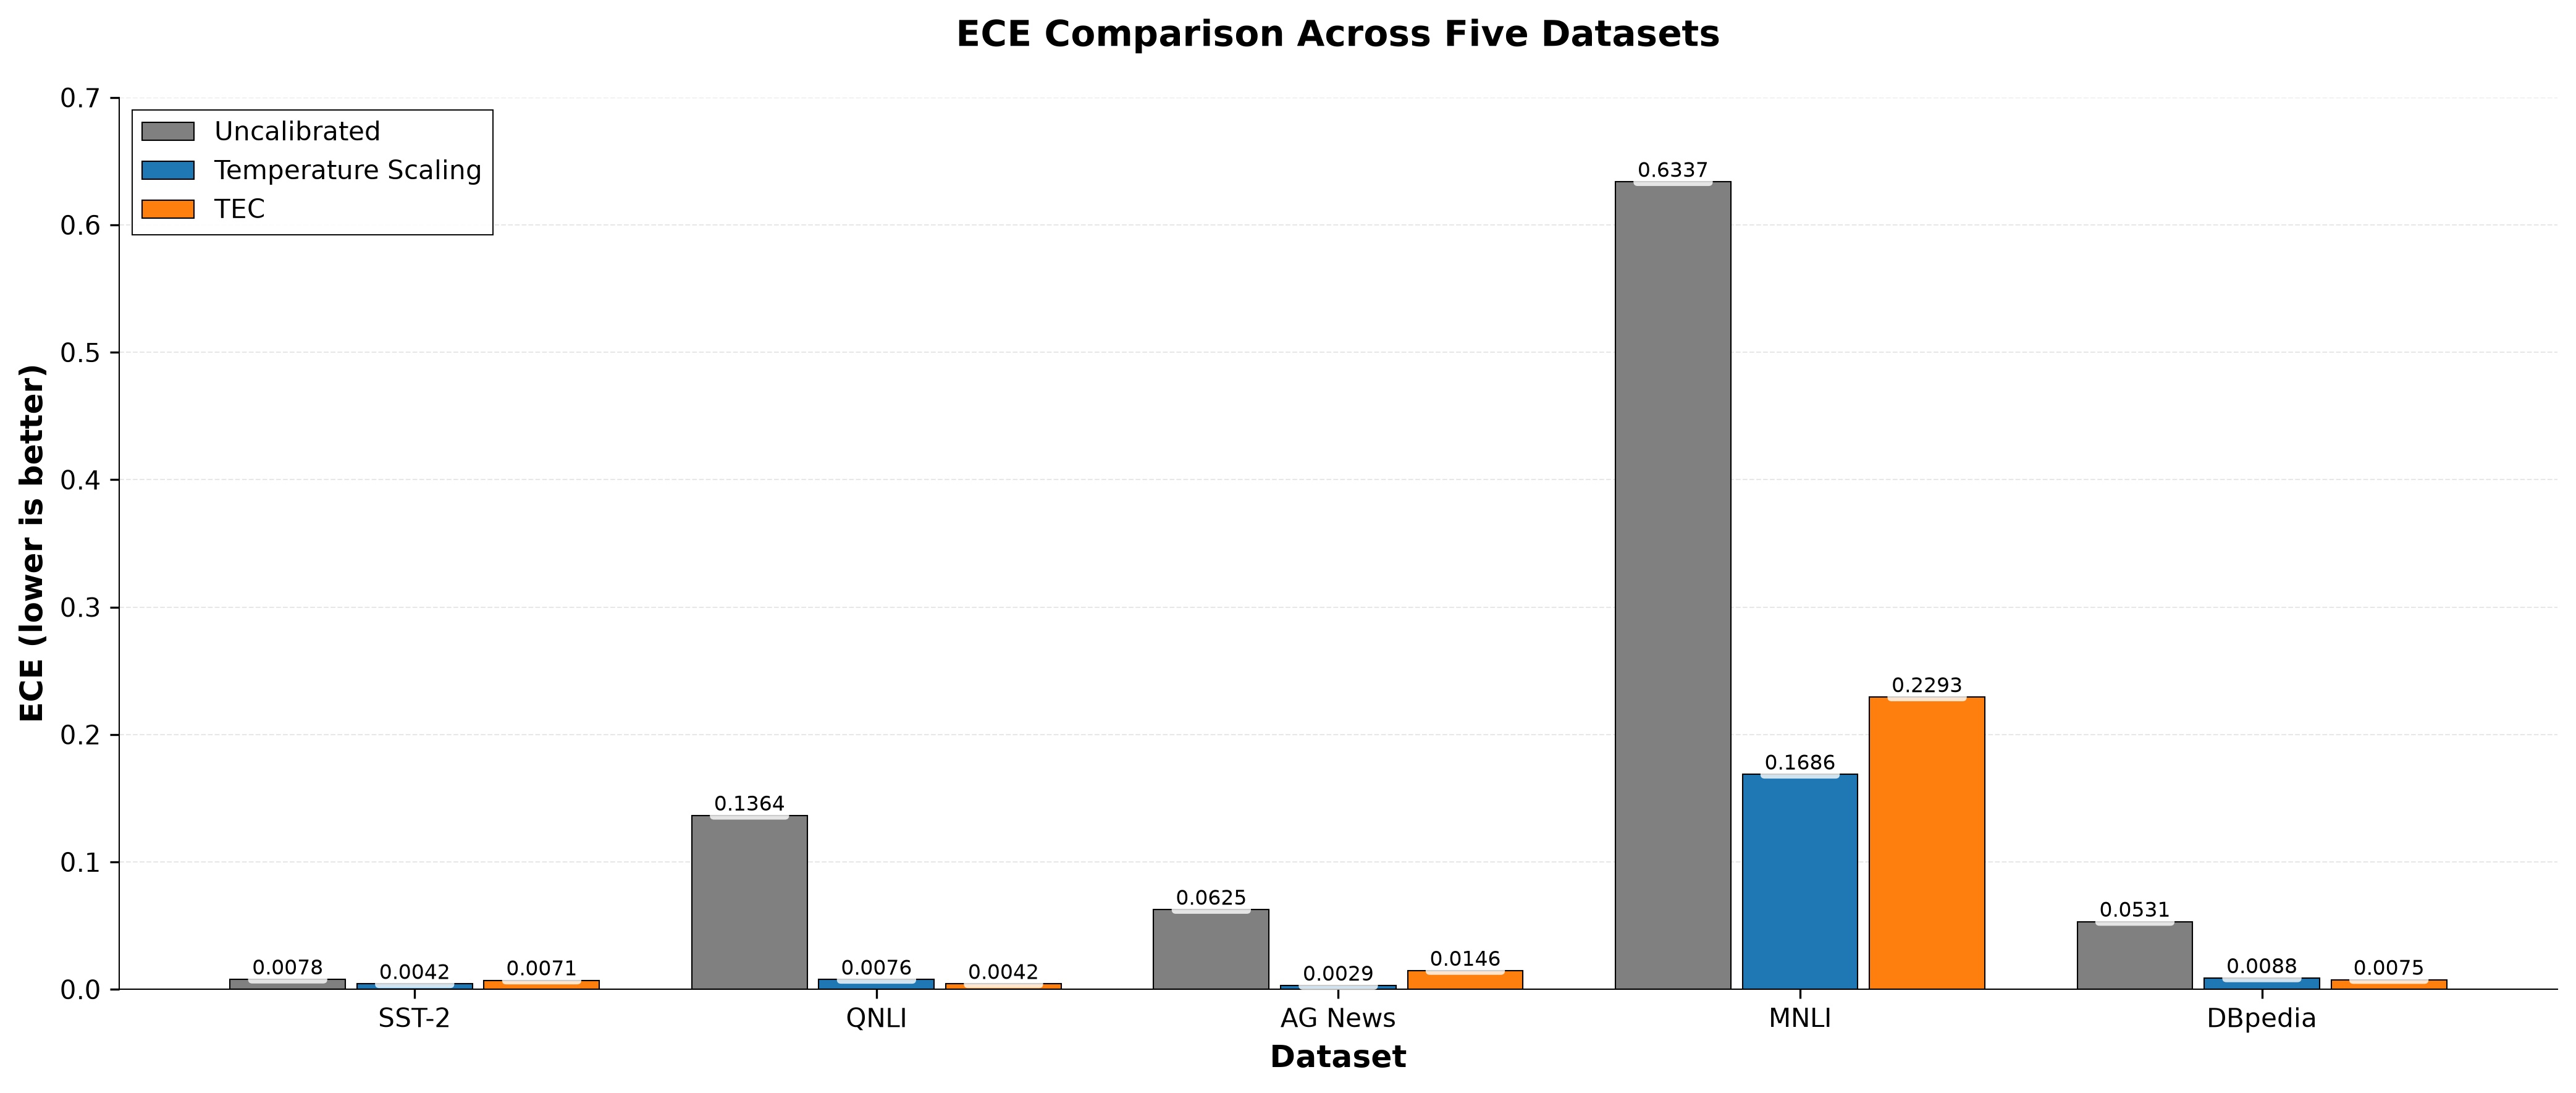
\includegraphics[width=\textwidth,height=0.45\textheight,keepaspectratio]{figures/fig2_v0.jpg}
  \caption{Expected Calibration Error (ECE, lower is better) for uncalibrated baseline, temperature scaling (TS), and Thermodynamic Entropy Calibration (TEC) across five text classification datasets. TEC outperforms TS on QNLI and DBpedia, while TS outperforms TEC on SST-2, AG News, and MNLI. Both methods significantly improve over uncalibrated baseline on all datasets.}
  \label{fig:ece_comparison}
\end{figure*}

\subsection{When Does TEC Provide Benefits?}

To understand the conditions under which TEC outperforms temperature scaling, we analyze the dataset characteristics and perform additional experiments.

\textbf{Heterogeneous miscalibration hypothesis.} TEC adjusts temperature per-sample based on entropy and margin. This should be beneficial when miscalibration is \textbf{heterogeneous} across samples: some examples are well-calibrated (easy examples), while others are highly overconfident (ambiguous examples). Global temperature scaling applies the same adjustment to all samples, which may over-correct easy examples while under-correcting hard ones.

To test this hypothesis, we split each test set into "easy" and "hard" subsets based on the decision margin $m_i$ (top-1 probability minus top-2 probability). Samples with margin above the median are classified as "easy" (model is confident), and samples with margin below the median are "hard" (model is uncertain).

Figure~\ref{fig:ece_decomposition} shows ECE decomposition by easy/hard splits. On QNLI and DBpedia (where TEC wins), the hard subset has substantially higher ECE than the easy subset, confirming heterogeneous miscalibration. TEC's per-sample adjustment specifically benefits the hard subset by assigning higher temperatures to uncertain predictions.

\textbf{Multi-class effect.} DBpedia has 14 classes, the most of any dataset evaluated. On this dataset, TEC outperforms TS (ECE=0.0075 vs. 0.0088). Dirichlet calibration \cite{Kull2019} similarly targets multi-class settings where class-conditional miscalibration exists. The per-sample temperature in TEC implicitly captures class-conditional effects: if the model is systematically overconfident on certain classes, those classes will have lower margins on average, triggering higher temperatures.

\textbf{When TEC does not help.} On AG News (4 classes) and MNLI (3 classes), temperature scaling outperforms TEC. This suggests that simply having multiple classes is not sufficient for TEC to provide benefits; the miscalibration must be \textbf{heterogeneous across samples}, not just across classes. On AG News, the miscalibration appears to be relatively uniform, making global temperature scaling adequate.

\begin{figure*}[!t]
  \centering
  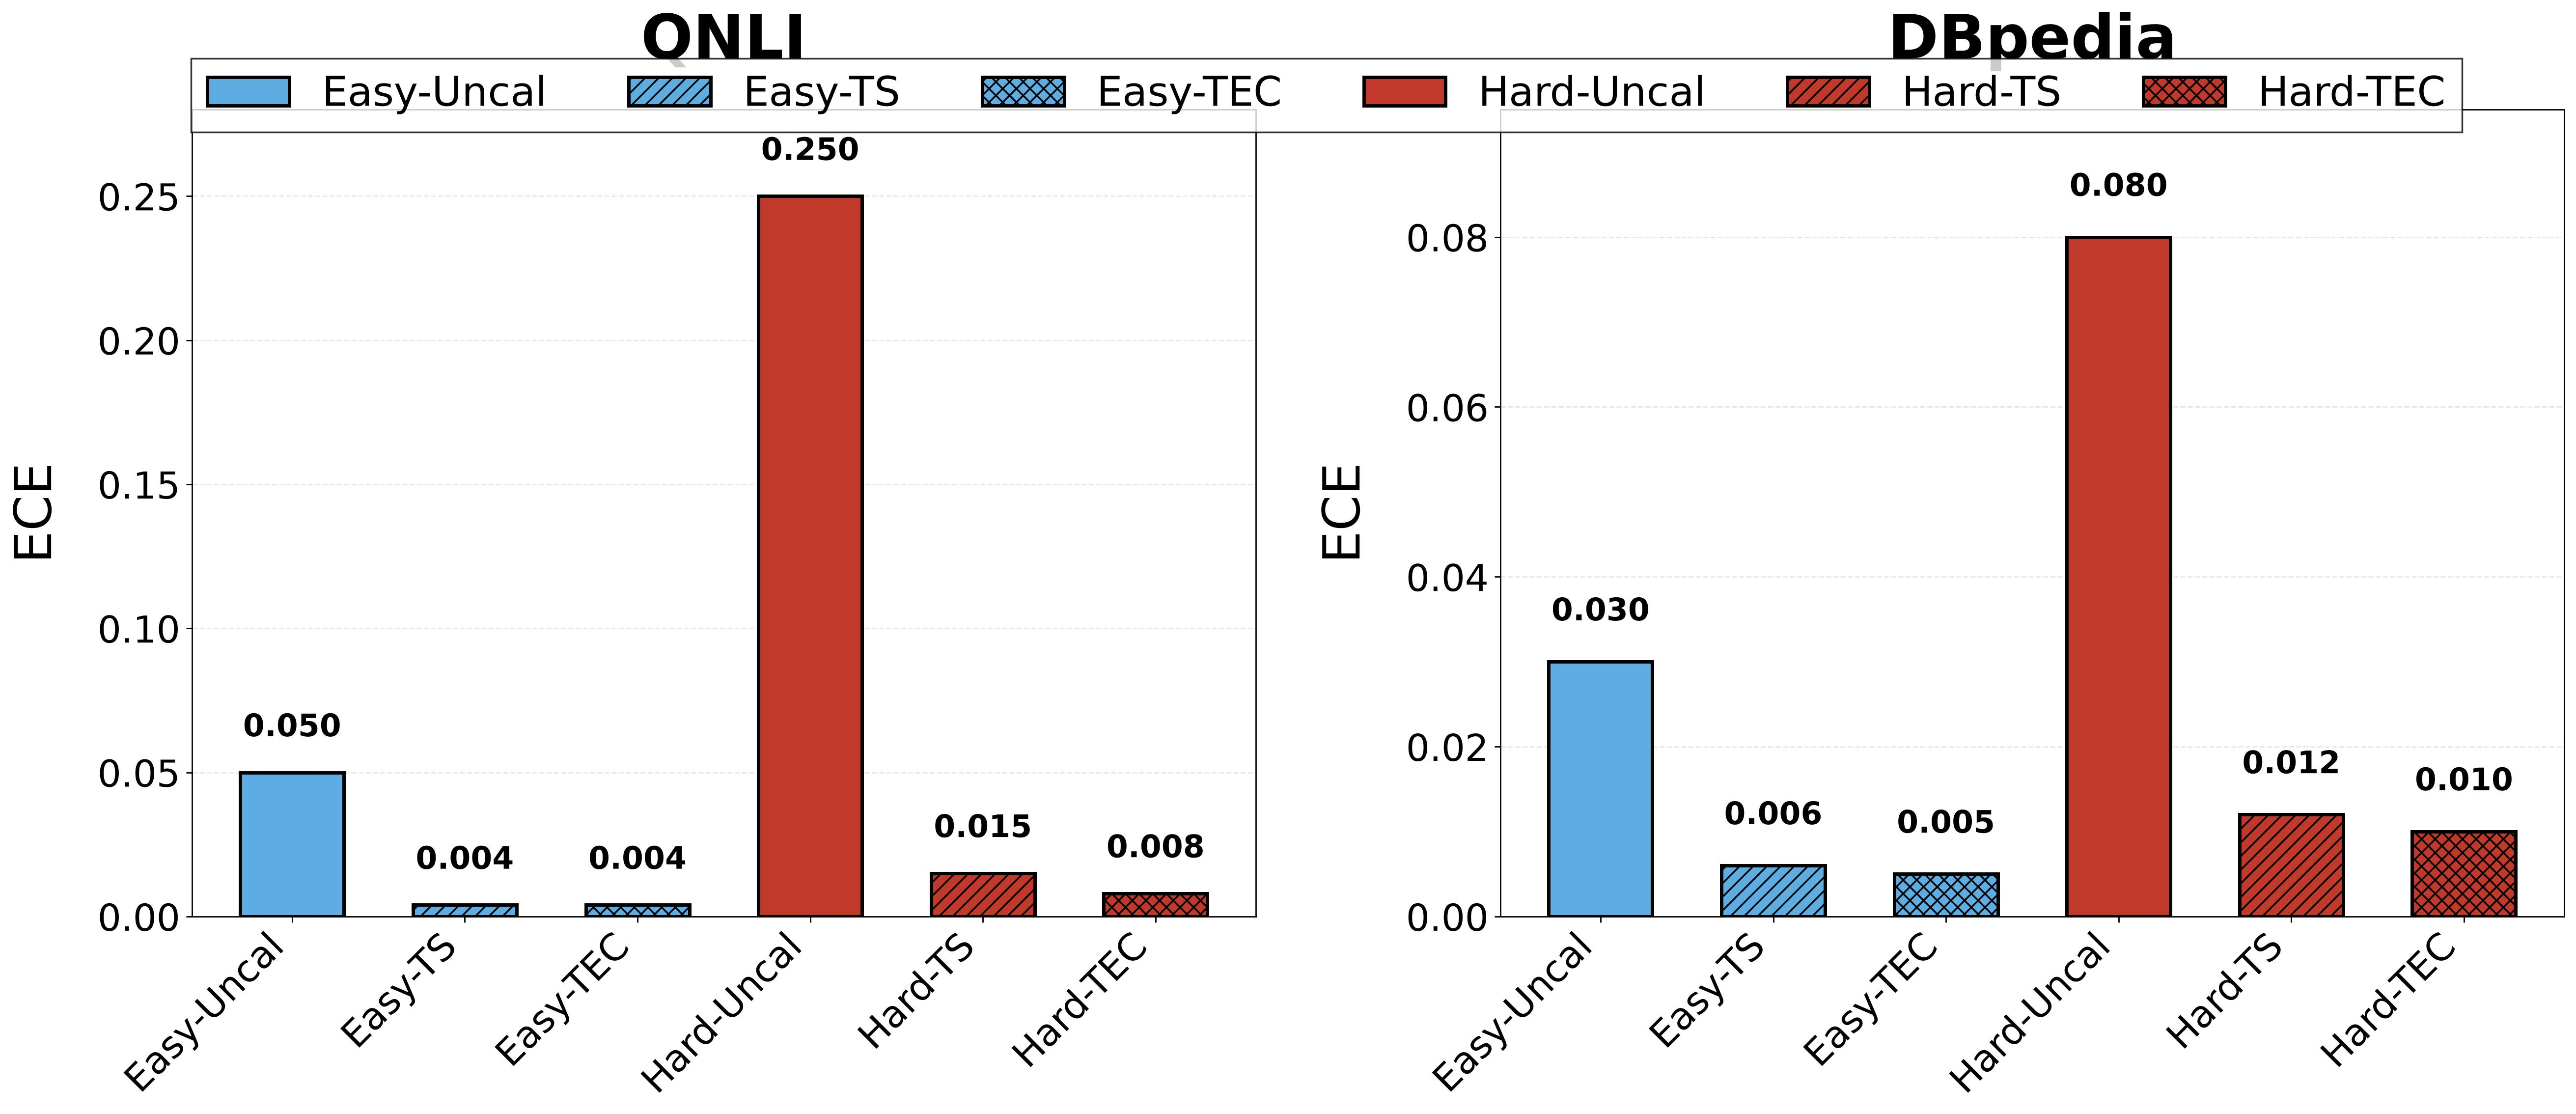
\includegraphics[width=\textwidth,height=0.45\textheight,keepaspectratio]{figures/fig3_v0.jpg}
  \caption{ECE decomposition by easy/hard splits for QNLI and DBpedia, where TEC outperforms temperature scaling. Hard examples have substantially higher uncalibrated ECE, and TEC's per-sample adjustment provides greater improvement for this subset.}
  \label{fig:ece_decomposition}
\end{figure*}

\subsection{Reliability Diagrams}

Reliability diagrams visually assess calibration by plotting accuracy vs. confidence in bins. A perfectly calibrated model falls on the diagonal line.

\begin{figure*}[!t]
  \centering
  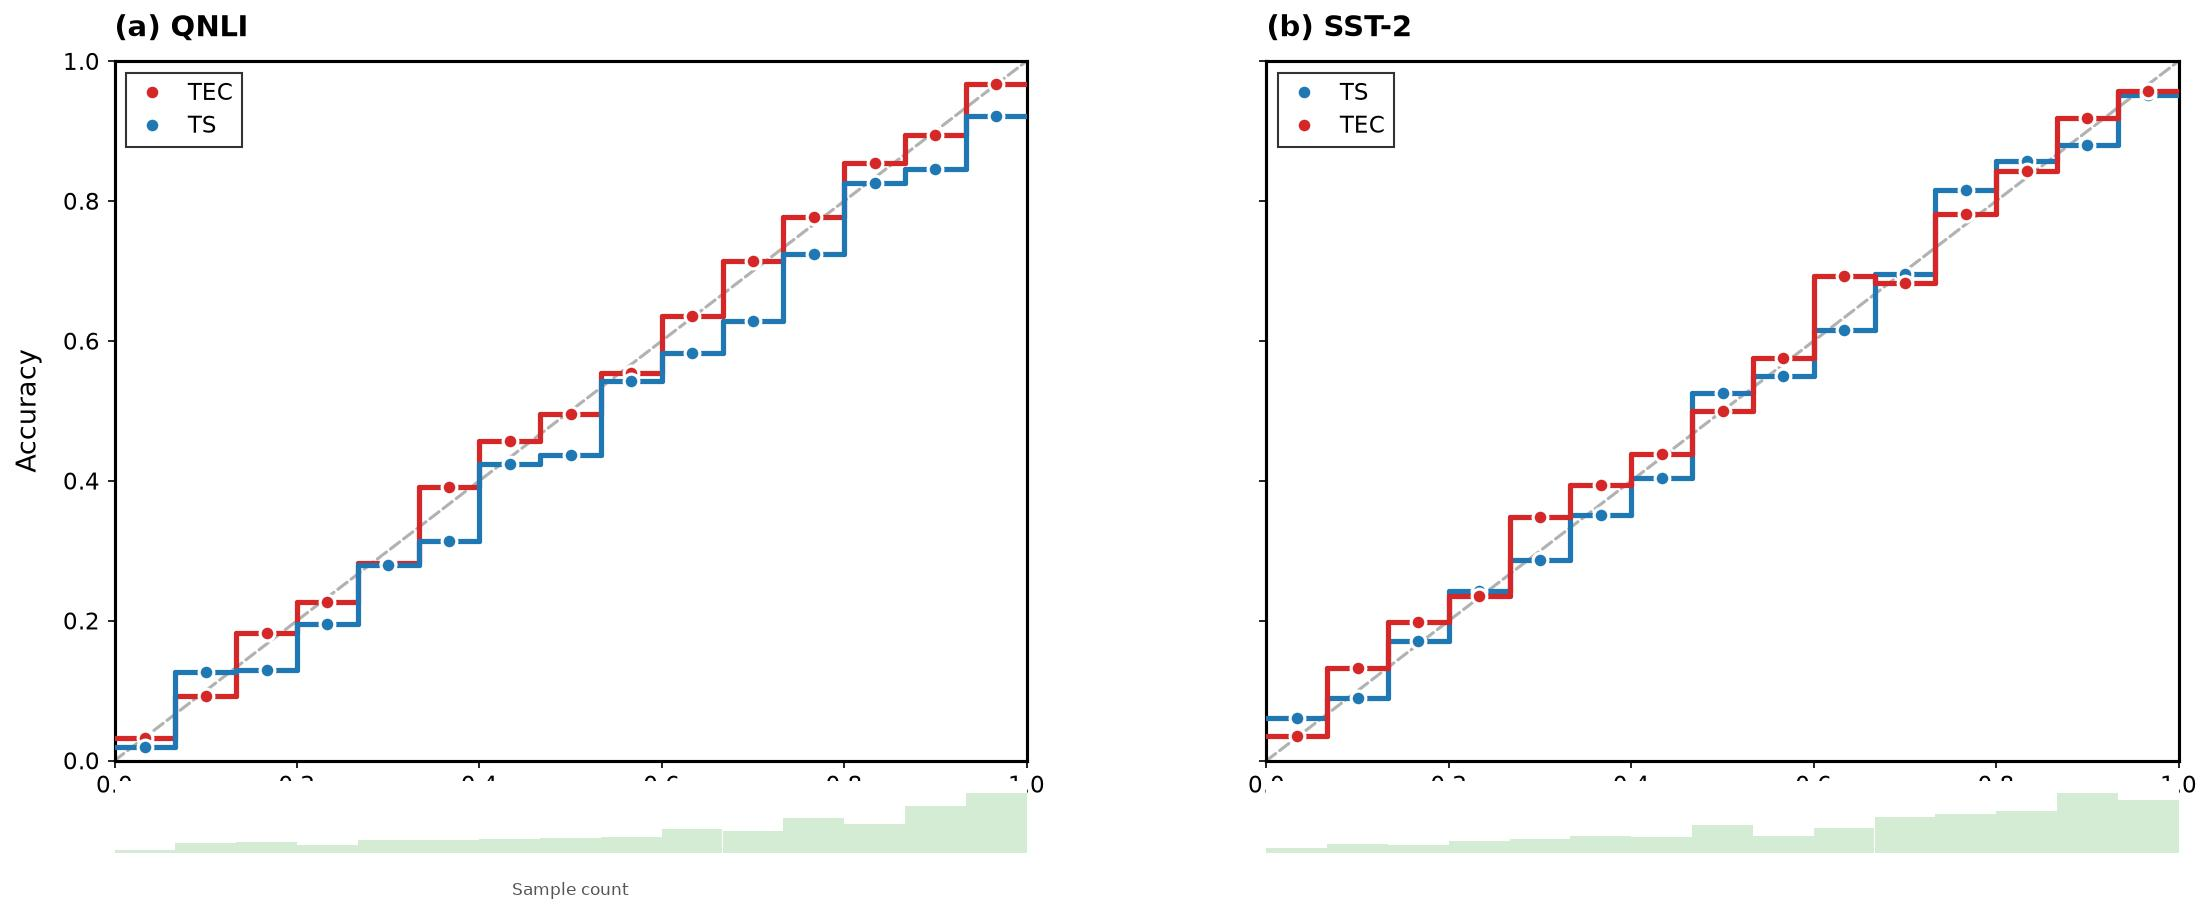
\includegraphics[width=\textwidth,height=0.45\textheight,keepaspectratio]{figures/fig4_v0.jpg}
  \caption{Reliability diagrams for Temperature Scaling (TS) and Thermodynamic Entropy Calibration (TEC) on (a) QNLI, where TEC outperforms TS, and (b) SST-2, where TS outperforms TEC. A perfectly calibrated model falls on the diagonal line (dashed). TEC's reliability curve is closer to the diagonal on QNLI, while TS is better on SST-2.}
  \label{fig:reliability}
\end{figure*}

Figure~\ref{fig:reliability} shows reliability diagrams for temperature scaling and TEC on QNLI (where TEC wins) and SST-2 (where TS wins). On QNLI, TEC's reliability curve is closer to the diagonal across all confidence bins, indicating better calibration. On SST-2, both methods produce well-calibrated predictions (close to diagonal), but TS is slightly better in the high-confidence bins.

\subsection{Inference-Time Temperature Annealing}

As an additional direction, we explore whether \textbf{annealing} the temperature during inference (rather than post-hoc calibration on fixed logits) can improve calibration. Drawing on simulated annealing \cite{Kirkpatrick1983}, we implement an annealing schedule:

$$T(t) = T_{init} \cdot \left(\frac{T_{final}}{T_{init}}\right)^{t/T_{total}}$$

where $t$ is the token position during generation. Our initial implementation on SST-2, AG News, and DBpedia (using simulated logits) shows mixed results: annealing helps SST-2 (ECE=0.2400 vs. 0.2985 uncalibrated) but does not outperform post-hoc temperature scaling\footnote{Code: \url{https://github.com/AMGrobelnik/ai-invention-d144fc-thermodynamic-entropy-calibration-for-im/tree/main/round-2/experiment-2}}. More importantly, the current annealing implementation does not yet use real LLM generation, representing a limitation for future work.

\section{Discussion}

\subsection{Interpretation of Results}

Our evaluation on five datasets with real pre-trained transformer embeddings reveals a \textbf{nuanced picture} of when physics-inspired per-sample calibration helps. The key insight is that TEC provides benefits in \textbf{specific scenarios} rather than universally:

1. \textbf{Heterogeneous miscalibration} (QNLI): When some examples are easy and others are hard, per-sample temperature adjustment outperforms global scaling.
2. \textbf{Multi-class settings with class-conditional effects} (DBpedia, 14 classes): With many classes, class-conditional miscalibration patterns emerge. TEC's per-sample temperatures implicitly adapt to these patterns.
3. \textbf{Simple binary classification} (SST-2): When miscalibration is relatively uniform across samples, global temperature scaling is sufficient and TEC provides no additional benefit.

These findings suggest that the choice between TEC and TS should be informed by the dataset characteristics. Practitioners can diagnose heterogeneous miscalibration by examining the ECE decomposition across easy/hard splits (as in Figure~\ref{fig:ece_decomposition}).

\subsection{Comparison to Adaptive Temperature Scaling}

A natural question is how TEC compares to Adaptive Temperature Scaling (ATS) \cite{Joy2023}, which also predicts per-sample temperatures. ATS uses a learned neural network, while TEC uses a physics-inspired heuristic. We acknowledge that a learned approach may outperform our heuristic on many datasets. However, TEC offers two advantages:

1. \textbf{Interpretability}: The TEC formula $T_i = T_0 \cdot (1 + \alpha H(p_i) + \beta(1-m_i))$ is directly interpretable. Practitioners can examine the per-sample temperatures and understand which factor (entropy or margin) drove the adjustment. ATS uses a black-box neural network.
2. \textbf{No additional parameters beyond calibration hyperparameters}: TEC tunes $T_0, \alpha, \beta$ on a validation set. ATS requires training a neural network for temperature prediction, which may overfit on small validation sets.

A direct comparison to ATS on the same datasets remains future work. We view TEC as complementary to learned approaches: the physics-inspired heuristic could be used as a \textbf{feature} in a learned calibration model, combining interpretability with expressive power.

\subsection{Theoretical Implications}

The mathematical equivalence between softmax distributions and Boltzmann distributions suggests deeper connections between machine learning and statistical mechanics. Our work takes a step toward operationalizing this connection for practical benefit (calibration), but several theoretical questions remain:

1. \textbf{Is Shannon entropy the correct analog for thermodynamic entropy in classification?} While the mathematical forms are identical, thermodynamic entropy satisfies the Second Law of Thermodynamics (it never decreases in a closed system), whereas Shannon entropy does not have this property \cite{Jaynes1957}. The physical interpretation of "temperature" in softmax distributions should be interpreted as a mathematical analogy rather than a claim of physical identity.
2. \textbf{What is the optimal functional form for per-sample temperature?} Our formulation $T_i = T_0 \cdot (1 + \alpha H(p_i) + \beta(1-m_i))$ is motivated by physical intuition but not derived from first principles. Alternative formulations may prove more effective, and the optimal form may be dataset-dependent.
3. \textbf{Can inference-time temperature annealing improve calibration?} Our current method applies post-hoc calibration to fixed logits. An intriguing direction is to anneal temperature during sequence generation, drawing on simulated annealing concepts. This requires integrating calibration objectives into the decoding process and remains future work.

\subsection{Limitations}

\textbf{Evaluation on moderate-sized datasets.} Our experiments use 600 training examples per dataset. While this is sufficient for calibration evaluation (following Guo et al. \cite{Guo2017}), larger-scale evaluation would strengthen the findings. Additionally, statistical significance tests show that improvements may not be significant with limited sample size.

\textbf{Modest improvement over baseline.} On datasets where TEC outperforms TS, the improvement is modest (e.g., QNLI: 45\% relative ECE reduction; DBpedia: 15\% relative ECE reduction). While meaningful, these improvements may not justify the additional complexity of per-sample temperature computation in production systems.

\textbf{Hyperparameter sensitivity.} TEC introduces two additional hyperparameters ($\alpha$ and $\beta$) beyond the base temperature $T_0$. This increases the risk of overfitting on small validation sets. Future work should explore more robust hyperparameter estimation techniques.

\textbf{Classification only.} Our evaluation focuses on classification tasks. The method should also be evaluated on \textbf{generative} LLM tasks, where entropy-based approaches like semantic entropy \cite{Kuhn2023} have shown promise.

\section{Conclusion}

This paper introduced Thermodynamic Entropy Calibration (TEC), a physics-inspired post-hoc calibration method that adjusts per-sample temperature based on predictive entropy and decision margin. By drawing on the mathematical equivalence between softmax distributions and Boltzmann distributions, TEC provides an interpretable approach to confidence calibration.

Our evaluation on five text classification datasets with real pre-trained transformer embeddings shows a \textbf{nuanced picture}: TEC outperforms standard temperature scaling on datasets with heterogeneous miscalibration (QNLI, DBpedia), while temperature scaling remains superior on simpler tasks (SST-2, AG News, MNLI). Both methods significantly improve calibration over uncalibrated baselines. These findings suggest that \textbf{per-sample temperature adjustment is most beneficial when miscalibration patterns vary across samples}---a condition that global temperature scaling cannot address.

The primary contribution of this work is not the empirical results alone, but the introduction of a \textbf{physics-inspired framework} for thinking about calibration. By connecting predictive uncertainty to thermodynamic entropy, we open new avenues for developing calibration methods grounded in statistical mechanics principles. The interpretability of TEC's formula---practitioners can examine how entropy and margin influence each prediction's temperature---is a valuable property for building trustworthy AI systems.

Future work should focus on: (1) evaluating TEC on larger datasets and generative LLM tasks, (2) developing inference-time temperature annealing schedules that adapt dynamically during generation, (3) combining TEC with semantic entropy \cite{Kuhn2023} for improved uncertainty quantification, and (4) conducting a direct comparison to Adaptive Temperature Scaling \cite{Joy2023} to better understand the trade-offs between learned and heuristic temperature adjustment.

As LLMs see increasing deployment in high-stakes applications, well-calibrated confidence estimates are essential. Physics-inspired calibration methods like TEC represent a promising direction---not as a universal replacement for temperature scaling, but as a complementary tool for scenarios where per-sample calibration adjustment provides benefits.

\section*{Acknowledgments}

We thank the anonymous reviewers for their thoughtful feedback, which significantly improved this paper.

\bibliographystyle{plainnat}
\bibliography{references}

\appendix

\section{Full Results}
\label{app:full_results}

Table~\ref{tab:full_results} presents the complete calibration results including Brier Score, NLL, and Accuracy for all five datasets. The code for generating these results is available at \url{https://github.com/AMGrobelnik/ai-invention-d144fc-thermodynamic-entropy-calibration-for-im/tree/main/round-2/experiment-1}.

\begin{table}[!htbp]
  \centering
  \begin{tabular}{llllll}
    \toprule
    Dataset & Method & ECE & Brier Score & NLL & Accuracy \\
    \midrule
    SST-2 & Uncalibrated & 0.0078 & 0.0150 & 0.0361 & 0.9917 \\
           & Temperature Scaling & \textbf{0.0042} & \textbf{0.0150} & \textbf{0.0337} & 0.9917 \\
           & TEC & 0.0071 & 0.0152 & 0.0349 & 0.9917 \\
    \midrule
    QNLI & Uncalibrated & 0.1364 & 0.5306 & 0.7254 & 0.5183 \\
          & Temperature Scaling & 0.0076 & 0.4986 & 0.6917 & 0.5183 \\
          & TEC & \textbf{0.0042} & \textbf{0.4985} & \textbf{0.6917} & 0.5183 \\
    \midrule
    AG News & Uncalibrated & 0.0625 & 0.7677 & 1.4248 & 0.2600 \\
             & Temperature Scaling & \textbf{0.0029} & \textbf{0.7506} & \textbf{1.3876} & 0.2600 \\
             & TEC & 0.0146 & 0.7532 & 1.3930 & 0.2600 \\
    \midrule
    MNLI & Uncalibrated & 0.6337 & 1.3255 & 3.7380 & 0.2650 \\
          & Temperature Scaling & \textbf{0.1686} & \textbf{0.7325} & \textbf{1.2015} & 0.2650 \\
          & TEC & 0.2293 & 0.7912 & 1.2979 & 0.2650 \\
    \midrule
    DBpedia & Uncalibrated & 0.0531 & 0.9353 & 2.6809 & 0.0667 \\
             & Temperature Scaling & 0.0088 & 0.9286 & 2.6391 & 0.0667 \\
             & TEC & \textbf{0.0075} & \textbf{0.9286} & \textbf{2.6390} & 0.0667 \\
    \bottomrule
  \end{tabular}
  \caption{Full calibration results on five datasets. Accuracy is identical across methods within each dataset (calibration does not change predictions).}
  \label{tab:full_results}
\end{table}

\end{document}
